\documentclass[main.tex]{subfiles}

\begin{document}

\chapter{Computing Background} \label{chapter:back}


\section{Parallel Computing}

Traditional computer programs are written in a sequential manner. It is natural to think of an algorithm as a sequence of steps that can be serially performed to achieve a final result. This has actually been the most common programming paradigm since the early days of computing, and it synergizes well with single processor machines. Optimizations related to instruction-level parallelism, such as out-of-order execution, pipelining, branch prediction or superscalarity, were mostly handled by the compiler or the hardware itself, and transparent to the programmer. Vector processing was also a key performance factor, allowing the same instruction to be simultaneously applied to a data vector, rather than one at a time (commonly referred to as \ac{SIMD}).

But in the beginning of the \rom{21} century, the development of computational chips shifted from a single faster core perspective, to a multi-core one. The evolution of single-core processors was already reaching its peak, and was slowing down due to the increasing difficulty in reducing transistor size or increasing clock frequencies, while introducing or aggravating other problems, such as heat dissipation, which becomes harder with the increased complexity of a chip. The solution was to move to a multi-core perspective, coupling more cores in the same chip, to share the workload and allow overall computational capabilities to keep evolving.

This has allowed hardware development to keep in conformance with Moore's Law. And while it was a necessary step from a hardware's perspective, this has important implications in software development. In order for an application to take advantage of multi-core technology, it needs to be broken into smaller tasks, that can be independently executed, usually with some form of synchronization and communication between them. Writing parallel algorithms requires an adaptation to this new paradigm, as a sequential line of execution does not provide efficient results in platforms that support parallel execution of several threads or processes.

Writing parallel algorithms is generally not a trivial task compared their sequential counterpart. Several classes of problems are introduced to the programmer such as deadlocks, data races and memory consistency. Some of these problems may cause applications to behave unexpectedly under certain conditions. That, along with the fact that multiple execution lines are being processed in a sometimes very loose order, is also what makes the debugging of these applications much harder.

This is not helped by the fact that current development environments are still mostly unequipped to aid the programmer in such tasks. Support for debugging and profiling is still somewhat outdated in various cases, as should be expected from a paradigm that has not become mainstream until recent years.


\section{The \gpu as a Computing Accelerator}

With the increasing demand for highly data-parallel algorithms, and the growing amount of data to process, hardware development started shifting towards the goal of solving that problem. Initially, that started with the increased support for vector instructions in common \cpus, and the \acs{SIMD} model. This allowed a single instruction to operate on a set of elements at once, effectively achieving a kind of parallelism which is extremely useful in data-parallel applications.

This data-parallel model is also behind the architecture of \gpus, but at a much higher degree. While the concept is the same (applying the same instruction to a set of values, instead of a single value at a time), the architecture of a \gpu, particularly a \cuda-enabled device, relies on the usage of several simple cores, grouped in multiple \aclp{SM}, to achieve higher degrees of parallelism, and process massive amounts of data.
These features makes \gpus more suitable for tasks with a high degree of data-parallelism, and not the ideal candidate for more irregular problems, where its more difficult to find parallelization points in order to take advantage of the \acs{SIMD} model.

Although the hardware of a \gpu is still tightly coupled with graphics processing and rendering, there have also been several advances in its usage as a general computing device (\acs{GPGPU}).

%%%%%%%%%%%%%%%%%%%%%%%%%%%%%%%%%%%%%%%
\subsection{Fermi Architecture}

The Fermi architecture was an important milestone of \gpus technology, as it was one of the first generations targeted directly towards \gpgpu and high performance computing, rather than purely graphics rendering. The first Fermi devices were released in 2010, and include more efficient support for double precision floating point number when compared to earlier generations. Fermi devices also included a GDDR5 memory controller with support for \ac{DMA} through the \acs{PCIe} bus, and up to 16 \acf{SM}, for a total of up to 512 \acs{CUDA} cores.

\image[width=0.6\textwidth]{arch_fermi}{Overview of the Fermi Architecture}{fig:fermi}

This architecture is backed by a hardware-based thread scheduler, within each \acs{SM}, that attempts to feed the execution unit with threads grouped in blocks of 32, or \textit{warps}. Since the scheduling is made directly via hardware, the switch between threads is nearly free, at least when compared with software scheduling on a \acs{CPU}. As a result, this strategy works better when the total amount of threads competing for resources is much higher than the amount of execution units, allowing for the latency of memory accesses to be hidden away by instantly scheduling a different \textit{warp}, effectively hiding memory latency while still keeping execution units busy. This is very different from \acs{CPU} scheduling policies, where switching between threads requires a context switch, which takes considerably longer, making that approach not as feasible as for a \gpu.


%%%%%%%%%%%%%%%%%%%%%%%%%%%%%%%%%%%%%%%%
\subsection{Kepler Architecture}

Kepler, the follow-up generation to Fermi, is in many ways similar to its predecessor. One of the most notorious change is the increase in the total amount of available CUDA cores, going up to 2880 in high-end devices due to the redesign of the \acl{SM}, now called \smx, each one with 192 \cuda cores. Kepler works at lower frequencies than Fermi, due to the removal of shader frequency, a compromise to make room for the extra \cuda cores. The entire chip now works based on the same core frequency. Overall, individual core efficiency is lowered, but the global system becomes more efficient.

\image[width=0.8\textwidth]{arch_kepler}{Overview of the Kepler Architecture}{fig:kepler}

The programming model has been extended with the addition of dynamic parallelism, allowing a \acs{CUDA} thread to spawn new threads, a feature not possible with previous \nvidia devices. This is a relevant feature for irregular algorithms. With Kepler we can also invoke multiple kernels for a single \gpu, transparently dividing them between the available \smxs.

This shows a clear evolution over the previous generation, and a response to the increasing demand for highly parallel computational power provided by \gpus.


\section{MIC Architecture}

\acf{MIC} \cite{Intel:MIC:QuickStartGuide} is an architecture proposed by \intel as a competitor to \gpus for general purpose high performance computing. This alterative device employs 61 cores with a micro-architecture similar to \textit{x86}, with a 1GHz frequency, and up to 16GB of GDDR5 memory, as well as two levels of cache. The last level is interconnected via a bidirectional ring among all cores, effectively sharing memory creating a last level cache with over 30MB.
While the \acs{MIC} architecture is based on the \textit{x86} that is used in common \cpus. Extensions to the micro architecture provide support for 64-bit addressing, and SIMD instructions are possible using 512-bit registers. However, instruction sets such as \acf{SSE} or \acf{AVX} are not compatible.

a \acs{MIC} device internally uses a Linux-based micro operating system, thus being able to run independently from the rest of the system, as opposed to other accelerating devices. This allows the device to operate in one of three possible modes:
\begin{description}
\item[Native] the device is used as an independent system, with applications running entirely on it;
\item[Offload] the host system uses the device as a coprocessor, by offloading specific tasks to it. This is the usual mode accelerators such as \cuda devices work;
\item[Message Passing] By using \acs{MPI}, the device can be used simply as another node in the network.
\end{description}

Initial claims suggest that this architecture has the ability of providing performance improvements to existing applications, with little to no effort from the programmer. The compatibility (to some degree) with \textit{x86} makes this somewhat possible, although some reports have questioned this claim, particularly when attempting to running native \textit{x86} application originally target at \xeon \cpus\cite{MIC:Nvidia}.


\section{Heterogeneous Platforms}

By combining multiple devices such as \cpus and \gpus, the obtained platform can obtain a much higher theoretical peak performance. But in practical terms, it becomes much harder, if not impossible at all, to achieve performances near this peak value.

On a homogeneous machine, the actual peak performance is limited by additional factors such as pipeline bubbles\footnote{A delay in the instruction pipeline, required to solve data, structure or control hazards, and limiting \ac{ILP} }, or memory access times, which is aggravated in memory bound algorithms \cite{williams2009roofline}.

When dealing with multiple devices with disjoint memory address spaces, an additional layer of complexity is introduced, as these different devices need a mean of communication between each other. Usually, a \hetplat, such as the one represented in \cref{fig:hetplat} can be seen as a distributed memory system, since each device has its own memory hierarchy. Communication is thus needed for synchronization between tasks, and for all required data transfers.

\begin{figure}[!htp]
  \centering
  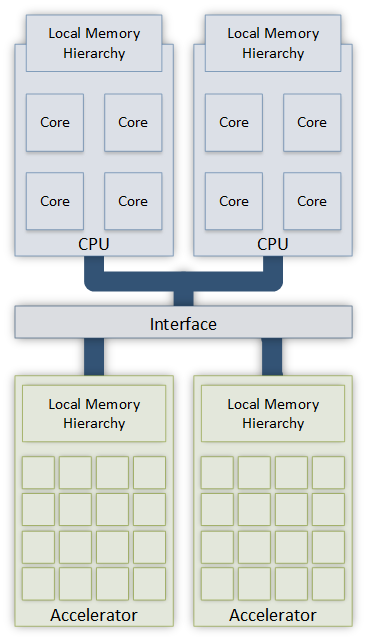
\includegraphics[width=0.3\textwidth]{visio/hetplats}
  \caption{Example diagram of a \hetplat \label{fig:hetplat}}
\end{figure}

In the case of \gpus, communication is done via a \acs{PCIe} bus. Although this technology has greatly evolved over the last recent years, this still proves to be a potential bottleneck for accelerating applications with a \gpu.

Even disregarding \acs{PCIe} devices, a single computational node can also be composed of multiple \cpu sockets, connected to each other via a bus such as \ac{QPI}. This bus connects not only the multiple sockets but also the memory banks possibly associated with each one, as these types of machines are generally associated with a \acs{NUMA} memory hierarchy, where each \cpu is directly connected to a different memory bank. While access to all banks is shared between all \cpus, access costs are not uniform. They depend on the bus bandwidth used, and also on the actual path a request has to make from the socket it originated from until it reaches the desired memory bank.

While this is a completely transparent process to the programmer, it can be another source of performance degradation, if most or all data might ends up pinned to a single memory bank, requiring all other sockets to share access to it. This is commonly disregarded by programmers, who end up treating these systems as if their main memory is unified. It is possible to control the affinity of both data and task in a \acs{NUMA} system. For instance, the \texttt{hwloc}\cite{broquedis2010hwloc} library provides access to the topology of the system, as well as an API to control their bindings, effectively allowing control over each individual \cpu and data bank.

However, libraries such as \texttt{hwloc} are very low-level ones, thus difficult to learn and use properly. For complex problems, worrying about low-level optimizations such as memory and core affinity can lead to over-optimization, making the application much more complex, less portable and harder to debug or modify.
Instead, these libraries should be used as a control layer for other libraries or frameworks to work on top of, and allowing a more developer-friendly access to the desired features.

\section{Heterogeneity and the Future}

As stated before, current \hetplats are usually composed with \cpus and \gpus communicating through a \acs{PCIe} slot. Newer technologies such as the \intel \mic also use this interconnect technique. Both these accelerators have their own memory hierarchy, different from the host \cpu, and the latter one is actually \textit{x86}-based, making it architecturally more similar to ordinary \cpus. However, as history has shown, this cannot be assumed as the global model for heterogeneous computation.

As an example, power efficiency has recently become a more prominent factor in technological evolution. Judging from that, it should be expected that short term evolution would yield more power efficient devices, rather that just providing a higher peak performance or increasing the number of cores. Power efficiency can also be regarded as a relevant factor by a scheduling framework, by making decisions not only based on overall execution time of the application, but also based on its costs in terms of energy consumption.
Other metrics can be though of, and their importance increased or decreased, depending on technological trends at each time.

In fact, in early 2013 AMD has already announced a new approach to heterogeneous computing, called \acs{hUMA}, which effectively implements a shared memory system between the host \cpu and a \gpu \cite{hUMA}. This eliminates the communication required between both devices through the \acs{PCIe} bus, which can lead to significant advances in performance. However, such as system will also be incompatible (or at least, not adequate) to any framework, or programming methodology, that assumes a distributed memory system, and the need of \acs{PCIe} communication.

All these factors emphasize the fact that optimizations based solely on architectural details (for example, software pre-fetching, core affinity and memory affinity) are not desirable to be coupled with an application if is desirable for it to perform well in future platforms, instead of becoming less performant. Such optimizations create tight dependencies between a program's performance, and the actual architecture(s) being used during development. So, it becomes desirable that such issues be handled by a more generic tool, built in a modular way, so that components can be plugged, unplugged or updated, and applications easily portable, while maintaining its efficiency.

\end{document}
